% =============================================================================
% COPYRIGHT AND DISCLAIMER
% =============================================================================
% This file is provided as a convenience template for competition participants.
% By using it, you accept full responsibility for compliance with all applicable
% copyright, licensing, and usage rules of the Association for Computing
% Machinery (ACM) and of any LaTeX packages you load (including, without
% limitation, the "acmart" document class and related ACM materials).
%
% Consult ACM's official publication, template, and copyright policies before
% using this setup for any purpose other than this competition. Do not assume
% that this template may be reused, redistributed, or submitted elsewhere
% without independently verifying ACM's current rules.
%
% Use of the "acmart" class, the "sigconf" option, or ACM-style formatting in
% this template does NOT mean that this report, this competition, its organizers,
% or any resulting PDF is sponsored, endorsed, affiliated with, or published by
% ACM. ACM trademarks and branding remain the property of ACM.
%
% Template packages live in preamble.tex.
% Citations live in main.bib. Edit this file with your paper content.
% =============================================================================

\documentclass[sigconf]{acmart}
% =============================================================================
% Template setup — participants normally do not edit this file.
% Author content belongs in main.tex; citations belong in main.bib.
% \documentclass lives in main.tex so Overleaf does not treat this file as root.
% =============================================================================

% --- Competition / non-ACM-submission friendly rights metadata -------------
\setcopyright{none}
\settopmatter{printacmref=false}
\acmConference[Kaggle Competition]{Filament Segmentation Challenge}{2026}{\href{https://www.kaggle.com/competitions/filament-segmentation-2026}{kaggle.com/competitions/filament-segmentation-2026}}
\acmBooktitle{Competition Report}
\acmDOI{}
\acmISBN{}

% --- Author guidance text --------------------------------------------------
% \guide{...} is gray italic while \guideStyletrue; omitted from the PDF if false.
% Flip the switch in main.tex after % =============================================================================
% Template setup — participants normally do not edit this file.
% Author content belongs in main.tex; citations belong in main.bib.
% \documentclass lives in main.tex so Overleaf does not treat this file as root.
% =============================================================================

% --- Competition / non-ACM-submission friendly rights metadata -------------
\setcopyright{none}
\settopmatter{printacmref=false}
\acmConference[Kaggle Competition]{Filament Segmentation Challenge}{2026}{\href{https://www.kaggle.com/competitions/filament-segmentation-2026}{kaggle.com/competitions/filament-segmentation-2026}}
\acmBooktitle{Competition Report}
\acmDOI{}
\acmISBN{}

% --- Author guidance text --------------------------------------------------
% \guide{...} is gray italic while \guideStyletrue; omitted from the PDF if false.
% Flip the switch in main.tex after % =============================================================================
% Template setup — participants normally do not edit this file.
% Author content belongs in main.tex; citations belong in main.bib.
% \documentclass lives in main.tex so Overleaf does not treat this file as root.
% =============================================================================

% --- Competition / non-ACM-submission friendly rights metadata -------------
\setcopyright{none}
\settopmatter{printacmref=false}
\acmConference[Kaggle Competition]{Filament Segmentation Challenge}{2026}{\href{https://www.kaggle.com/competitions/filament-segmentation-2026}{kaggle.com/competitions/filament-segmentation-2026}}
\acmBooktitle{Competition Report}
\acmDOI{}
\acmISBN{}

% --- Author guidance text --------------------------------------------------
% \guide{...} is gray italic while \guideStyletrue; omitted from the PDF if false.
% Flip the switch in main.tex after \input{preamble}.
%
% Do not use \guide{...} for \email{...}.
\usepackage{xcolor}
\newif\ifguideStyle
\guideStyletrue
\newcommand{\guide}[1]{%
  \ifguideStyle
    {\color{gray!65}\itshape #1}%
  \fi
}

% --- Math ------------------------------------------------------------------
% Do NOT load amssymb (or amsfonts): acmart already loads newtxmath, which
% defines the same symbols (e.g. \Bbbk) and causes a conflict on Overleaf.
% amsmath is already provided by acmart; mathtools extends it.
\usepackage{mathtools}

% --- Figures ---------------------------------------------------------------
% graphicx is already loaded by acmart
\usepackage{subcaption}

% --- Tables ----------------------------------------------------------------
% booktabs is already loaded by acmart
\usepackage{tabularx}
\usepackage{multirow}

% --- Bibliography style is set in main.tex (ACM-Reference-Format) ----------
.
%
% Do not use \guide{...} for \email{...}.
\usepackage{xcolor}
\newif\ifguideStyle
\guideStyletrue
\newcommand{\guide}[1]{%
  \ifguideStyle
    {\color{gray!65}\itshape #1}%
  \fi
}

% --- Math ------------------------------------------------------------------
% Do NOT load amssymb (or amsfonts): acmart already loads newtxmath, which
% defines the same symbols (e.g. \Bbbk) and causes a conflict on Overleaf.
% amsmath is already provided by acmart; mathtools extends it.
\usepackage{mathtools}

% --- Figures ---------------------------------------------------------------
% graphicx is already loaded by acmart
\usepackage{subcaption}

% --- Tables ----------------------------------------------------------------
% booktabs is already loaded by acmart
\usepackage{tabularx}
\usepackage{multirow}

% --- Bibliography style is set in main.tex (ACM-Reference-Format) ----------
.
%
% Do not use \guide{...} for \email{...}.
\usepackage{xcolor}
\newif\ifguideStyle
\guideStyletrue
\newcommand{\guide}[1]{%
  \ifguideStyle
    {\color{gray!65}\itshape #1}%
  \fi
}

% --- Math ------------------------------------------------------------------
% Do NOT load amssymb (or amsfonts): acmart already loads newtxmath, which
% defines the same symbols (e.g. \Bbbk) and causes a conflict on Overleaf.
% amsmath is already provided by acmart; mathtools extends it.
\usepackage{mathtools}

% --- Figures ---------------------------------------------------------------
% graphicx is already loaded by acmart
\usepackage{subcaption}

% --- Tables ----------------------------------------------------------------
% booktabs is already loaded by acmart
\usepackage{tabularx}
\usepackage{multirow}

% --- Bibliography style is set in main.tex (ACM-Reference-Format) ----------

\usepackage{tikz}
\usetikzlibrary{positioning,arrows.meta}

% Guide styling: \guideStyletrue = show gray italic hints; \guideStylefalse = omit them
\guideStylefalse

\begin{document}

\title{Native-Resolution ConvNeXt U-Net with Hysteresis Instances and a Crop Refiner}
\subtitle{A Solution to the Solar Filament Segmentation Challenge 2026} % DO NOT CHANGE

% TODO(author): replace the name and email below with your own before submitting.
\author{AUTHOR NAME}
\affiliation{%
  \country{COUNTRY}
}
\email{author@example.com}

\begin{abstract}
    This report describes our solution to the Solar Filament Segmentation Challenge~2026, a Kaggle competition on automatic segmentation of solar filaments in GONG H-$\alpha$ observations. We predict a per-pixel filament probability with a U-Net whose ConvNeXt-Base encoder runs on the full $2048^2$ disk, turn it into instances with a hysteresis rule tuned directly for Panoptic Quality (PQ), and redraw every instance with a second, crop-level U-Net. All choices were made on out-of-fold predictions over the 707 training images, with folds grouped by observation date. The pipeline reaches an out-of-fold PQ of 0.451 (95\% bootstrap interval 0.442--0.460) and 0.39 on the public leaderboard, without any external annotations. Code, weights and a notebook that reproduces the submission are public.
\end{abstract}

\maketitle

% ==================================== %
%              INTRODUCTION            %
% ==================================== %
\section{Introduction}
    This report goes over the details of our submitted solution to the Solar Filament Segmentation Challenge~2026 \cite{filament-segmentation-2026}. The challenge, launched on July~10,~2026, is organized by the Earth-Space AI Research (ESAIR) Lab\footnote{\href{https://www.esairlab.com/home}{www.esairlab.com/}}. This challenge utilizes the MAGFiLO dataset for evaluation of the segmentation algorithms \cite{ahmadzadeh2024dataset}.

    The score is Panoptic Quality \cite{kirillov2019panoptic}, $\mathrm{PQ} = \sum_{\mathrm{TP}} \mathrm{IoU} / (|\mathrm{TP}| + \tfrac12|\mathrm{FP}| + \tfrac12|\mathrm{FN}|)$, where a prediction and a ground-truth filament match when their IoU exceeds 0.5. Each annotator's record of an image is scored on its own. Two properties of the task shaped our design. First, every split, merged or doubtful instance costs score, so deciding \emph{which} components to output matters as much as the mask quality. Second, the 707 training images carry 1,154 annotator records that often disagree, so the labels are noisy and the attainable PQ is far below 1. Our solution is deliberately simple: a strong semantic model, a PQ-tuned instance rule, and a local refiner. We used no data beyond the competition training set.

% ==================================== %
%              METHODOLOGY             %
% ==================================== %
\section{Methodology}\label{sec:methodology}

\begin{figure*}[t]
  \centering
  \begin{tikzpicture}[node distance=4mm and 5mm, font=\footnotesize,
      box/.style={draw, rounded corners=2pt, align=center, minimum height=11mm, inner sep=3pt, fill=gray!6},
      hl/.style={box, fill=blue!8}, >={Stealth[length=2mm]}]
    \node[box] (in) {H-$\alpha$ image\\$2048^2$ JPEG};
    \node[box, right=of in] (pre) {disk\\normalisation};
    \node[hl, right=of pre] (s1) {Stage 1: U-Net\\ConvNeXt-Base, $2048^2$\\2 seeds $\times$ folds, D4 TTA};
    \node[box, right=of s1] (p) {filament\\probability $p$};
    \node[box, right=of p] (inst) {hysteresis instances\\$p\geq0.4$, close 3 px\\peak $\geq0.7$, mean $\geq0.85$\\area $\geq200$ px};
    \node[hl, right=of inst] (s2) {Stage 2: refiner\\R34 U-Net on $256^2$ crops\\(image, $p$, seed mask)};
    \node[box, right=of s2] (out) {non-overlapping\\instances\\$\rightarrow$ RLE};
    \foreach \a/\b in {in/pre, pre/s1, s1/p, p/inst, inst/s2, s2/out} \draw[->] (\a) -- (\b);
  \end{tikzpicture}
  \caption{Inference pipeline. Blue boxes are learned; all thresholds are tuned on out-of-fold PQ.}
  \Description{Flow diagram: image, disk normalisation, stage-1 U-Net, probability map, hysteresis instance extraction, stage-2 crop refiner, non-overlapping instances.}
  \label{fig:pipeline}
\end{figure*}

\subsection{Data, targets and validation}
    The training set has 707 physical images ($2048^2$ grayscale) and 1,154 annotator records with about seven filaments per record. For the semantic model we use a \emph{soft} target: the mean over an image's records of each record's union mask. Pixels marked by every annotator get 1 and contested pixels get fractional values, which uses all the records instead of picking one. Images are split into five folds \emph{grouped by observation date}, because the GONG network observes the same Sun from several sites within minutes and near-duplicate frames would otherwise leak across folds. Every model, threshold and design choice below was selected on the out-of-fold (OOF) predictions of all 707 images, scored with our re-implementation of the organisers' self-evaluation code (PQ pooled over all 1,154 records). The public leaderboard (180 test images) served only as a second check.

\subsection{Pre-processing}
    Each image is converted to float and normalised by the mean and standard deviation of the solar disk (pixels brighter than 10\% of the maximum). Off-disk pixels are set to 0. We work at the native $2048^2$ resolution: filaments are often only a few pixels wide, and moving from $1024^2$ to native resolution was worth about +0.01 OOF PQ.

\subsection{Stage 1: semantic U-Net}
    We use a U-Net \cite{ronneberger2015unet} from \texttt{segmentation-models-pytorch} \cite{smp} with an ImageNet-pretrained ConvNeXt-Base encoder \cite{liu2022convnext} from \texttt{timm} \cite{timm}, a single input channel and one output logit. Training draws random $1024^2$ crops of the full-resolution images with a random dihedral (D4) transform, batch size 2, AdamW \cite{loshchilov2019adamw} (learning rate $10^{-4}$, weight decay $10^{-4}$, 5\% warm-up, cosine decay) for 10k steps in mixed precision. The loss is binary cross-entropy plus $\tfrac12$ soft Dice against the soft target. One model is trained per fold (about 80 minutes on a Kaggle T4). At test time each model predicts the whole $2048^2$ image under the 8 D4 transforms. The final model averages two training seeds: seed 0 (5 folds) and seed 1 (folds 0--3, 8k steps).

\subsection{Instance extraction}
    Instances are the 8-connected components of $\{p \geq t_{\mathrm{lo}}\}$ after a morphological closing of radius $r$ and hole filling. A component is kept only if its peak probability is $\geq t_{\mathrm{hi}}$, its mean probability is $\geq m$ and its area is $\geq a$. Because PQ charges $\tfrac12$ for every false positive, the mean-probability filter is the most important: it drops faint, doubtful components. The parameters were grid-searched on OOF PQ: $t_{\mathrm{lo}}=0.4$, $r=3$\,px, $t_{\mathrm{hi}}=0.7$, $m=0.85$, $a=200$\,px. Components are disjoint, so predictions never overlap.

\subsection{Stage 2: crop refiner}
    Each kept instance is redrawn locally. A square window around its bounding box (box plus 32\,px margin, at least 128\,px) is resized to $256^2$ with three channels: normalised image, stage-1 probability, and the instance's own mask. A ResNet-34 U-Net predicts the instance's mask in the window. Its target is the mean of the ground-truth masks matched to the instance (IoU $>0.5$) across the image's records. The refiner is trained out of fold: the model for fold $k$ only sees instances from the other folds' images, whose stage-1 maps are themselves out of fold. Training uses AdamW (one-cycle schedule, peak $3\times10^{-4}$), batch 32 and 4k steps with D4 augmentation, about 20 minutes per fold on a 4\,GB laptop GPU. At test time the five fold refiners and 8 D4 views are averaged, and the result is thresholded at 0.45 and pasted back at $2048^2$. Instances are processed in decreasing mean probability, and a pixel already claimed by an earlier instance is removed, so the output stays non-overlapping. Figure~\ref{fig:examples} shows typical results.

\begin{figure}[t]
  \centering
  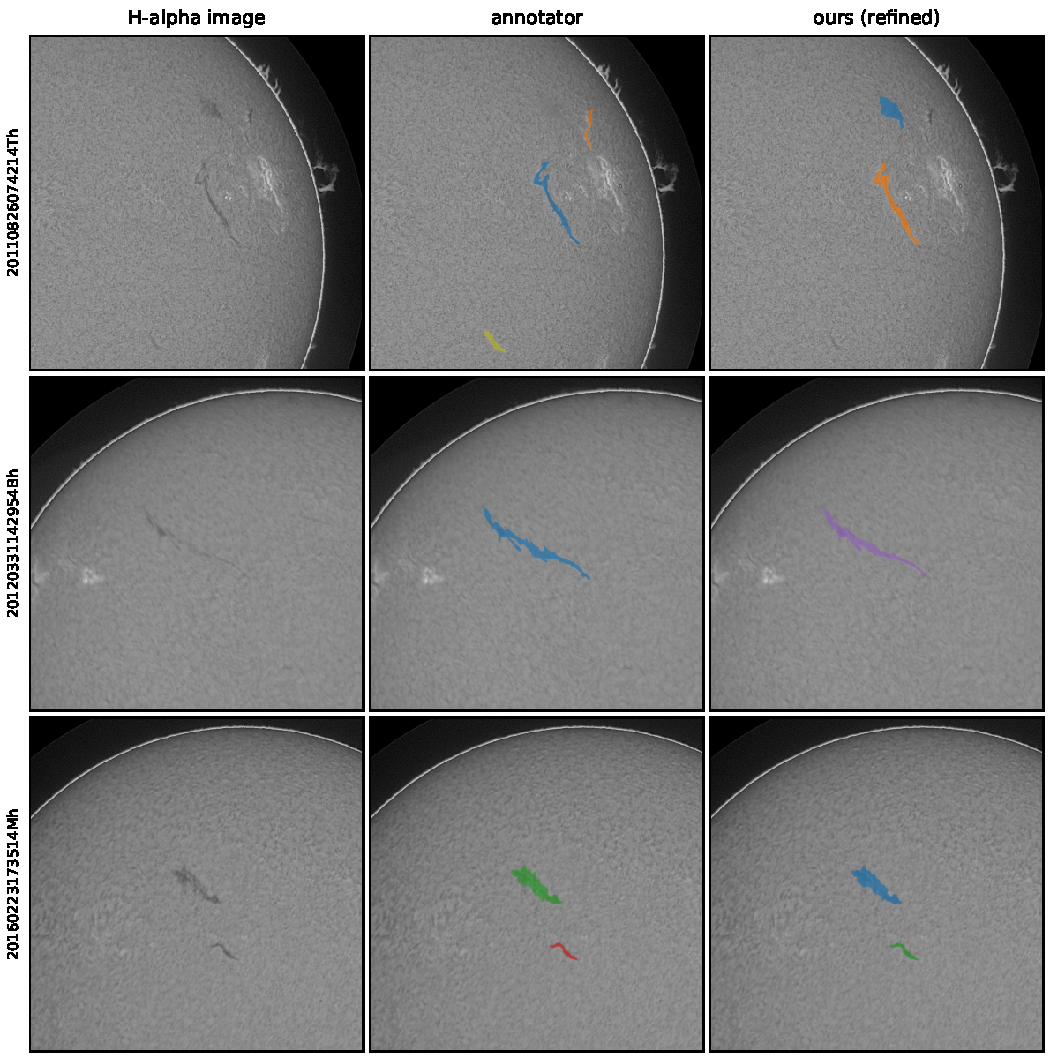
\includegraphics[width=\linewidth]{figures/qualitative.pdf}
  \caption{Out-of-fold examples ($1024^2$ windows). Colours separate instances. Row 3 shows a typical disagreement: the annotator split a filament where our model keeps one, and the reverse.}
  \Description{Three rows of image crops: the H-alpha image, the annotator's filament instances and our predicted instances.}
  \label{fig:examples}
\end{figure}

% ==================================== %
%              EVALUATION              %
% ==================================== %
\section{Evaluation}\label{sec:evaluation}

\subsection{Strategy}
    We report PQ over the OOF predictions of all 707 images and 1,154 records, which is the same pooled computation as the challenge metric. Uncertainty is given in two ways: the standard deviation of PQ across the five date-grouped folds, and a 95\% bootstrap interval obtained by resampling images ($B=2000$; all records of an image move together). For the refiner we bootstrap the \emph{paired} difference on the same images. Public leaderboard scores (180 test images, shown to two decimals) are listed for reference. Throughout the competition they sat about 0.05--0.06 below OOF, with the same ranking.

\subsection{Results}
    Table~\ref{tab:progress} traces the development. The largest gains came from treating the problem as semantic segmentation with a PQ-tuned instance rule, not as direct instance segmentation (YOLO11-seg \cite{yolo11}), from native resolution, and from a stronger encoder. Table~\ref{tab:stats} breaks down the final OOF result. The refiner improves PQ by $+0.0027$ (95\% interval $[+0.0005, +0.0048]$; 0.95\% of bootstrap draws $\leq 0$) and helps in four of five folds. Almost all of the gain is in segmentation quality (SQ $0.681\rightarrow0.685$; Figure~\ref{fig:iou}). Detection (RQ) is nearly unchanged, as expected, since the refiner redraws instances but does not select them. Averaging two seeds adds a further $+0.0022$ on folds 0--3 (0.4474 $\rightarrow$ 0.4496).

\begin{table}[t]
  \centering
  \caption{Development history: OOF PQ (707 images) and public leaderboard. $^\dagger$hold-out fold 0 only; $^\ddagger$folds 0--3.}
  \label{tab:progress}
  \small
  \begin{tabular}{@{}lcc@{}}
    \toprule
    Model & OOF PQ & Public \\
    \midrule
    YOLO11m-seg, $1024^2$ & 0.313$^\dagger$ & 0.28 \\
    U-Net R34, $1024^2$, soft target, hysteresis & 0.417 & 0.35 \\
    U-Net EfficientNet-B4, $1024^2$ & 0.422 & 0.36 \\
    U-Net EfficientNet-B4, native $2048^2$ & 0.433 & 0.37 \\
    U-Net ConvNeXt-Base, native $2048^2$ & 0.448 & 0.39 \\
    \quad + crop refiner & \textbf{0.451} & 0.39 \\
    \quad 2 seeds, before refiner & 0.450$^\ddagger$ & -- \\
    \quad 2 seeds + crop refiner (final) & -- & 0.39 \\
    \bottomrule
  \end{tabular}
\end{table}

\begin{table}[t]
  \centering
  \caption{OOF breakdown of the final instance rule without and with the refiner (all 1,154 records). Fold std.\ is over the five date-grouped folds; the interval is a 95\% image bootstrap.}
  \label{tab:stats}
  \small
  \begin{tabular}{@{}lcc@{}}
    \toprule
     & hysteresis & + refiner \\
    \midrule
    PQ & 0.4479 & \textbf{0.4505} \\
    \quad 95\% interval & [0.439, 0.457] & [0.442, 0.460] \\
    \quad fold mean $\pm$ std & $0.447 \pm 0.012$ & $0.450 \pm 0.011$ \\
    SQ (mean IoU of matches) & 0.681 & 0.685 \\
    RQ & 0.657 & 0.658 \\
    TP / FP / FN & 5172 / 2367 / 3027 & 5173 / 2357 / 3026 \\
    Dice of matches, mean (median) & 0.807 (0.815) & 0.810 (0.817) \\
    Splits (one GT $\rightarrow$ $\geq$2 preds) & 338 & 331 \\
    Merges (one pred $\rightarrow$ $\geq$2 GT) & 166 & 163 \\
    \bottomrule
  \end{tabular}
\end{table}

\begin{figure}[t]
  \centering
  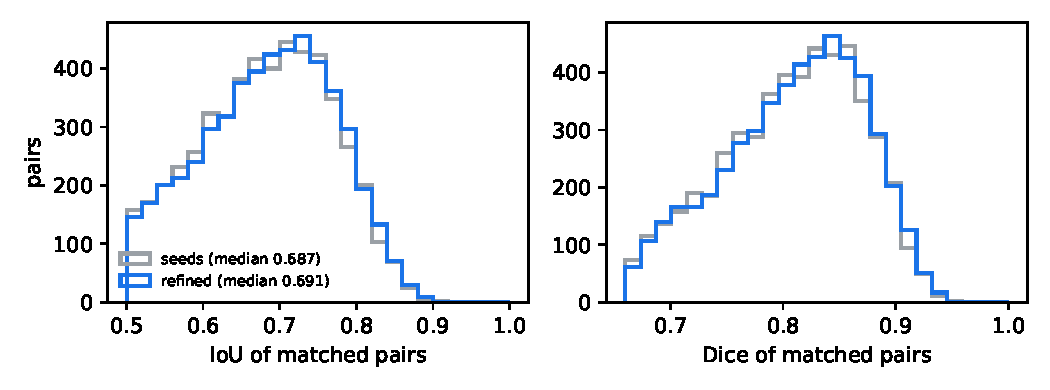
\includegraphics[width=\linewidth]{figures/iou_dice.pdf}
  \caption{IoU and Dice of matched (TP) pairs, OOF. The refiner shifts the distribution to the right.}
  \Description{Two histograms of IoU and Dice of matched pairs, for hysteresis seeds and refined masks.}
  \label{fig:iou}
\end{figure}

\subsection{What did not help}
    Several ideas were tested on OOF and dropped:
    \begin{itemize}
        \item Photometric and geometric augmentation beyond D4 (rotation, scale, contrast, blur, noise): $-0.022$ on folds 0--1.
        \item DINOv3-pretrained ConvNeXt weights \cite{simeoni2025dinov3}: $-0.018$; in an ensemble with the ImageNet model, $-0.004$.
        \item Averaging ConvNeXt with weaker encoders (EfficientNet-B4): no gain.
        \item A learned instance scorer over a threshold ladder, choosing components by gradient boosting with an exact tree DP: below the hysteresis rule.
        \item Learned merging of fragments across gaps: $+0.002$ OOF, no change on the leaderboard.
        \item Special handling near the limb: no gain.
    \end{itemize}

\subsection{Strengths, weaknesses and improvements}
    \textbf{Strengths.} The pipeline is short, deterministic at inference, and produces non-overlapping instances by construction. Splits and merges are rare: 331 and 163 against 8,199 ground-truth instances, about 4\% and 2\%. OOF estimates were stable across folds (std 0.011) and tracked the public leaderboard.
    \textbf{Weaknesses.} Recall is the main loss: 37\% of ground-truth instances are missed, mostly small, faint filaments that we suppress on purpose because a doubtful instance costs as much as a miss. The labels themselves limit the score: on images with several annotators, PQ between annotators was roughly 0.45--0.6 in our checks, so a large part of the remaining gap is label disagreement. Long filaments with faint gaps are sometimes split differently from the annotators (Figure~\ref{fig:examples}).
    \textbf{Improvements.} Training the refiner to also reject false positives (a learned selection step), larger encoders (ConvNeXt-Large fits a T4 with gradient checkpointing but exceeded our compute budget), and a loss that models annotator disagreement explicitly.

\subsection{Reproducibility and data use}
    The repository contains the training code, the trained weights (as release assets), \texttt{requirements.txt}, and a notebook that rebuilds the submission from the weights in about one hour on two T4 GPUs. We used only the competition training data and ImageNet-pretrained encoders. The public MAGFiLO release also contains annotations for the challenge's test images, so we never downloaded or used any external annotations.

% ==================================== %
%            ACKNOWLEDGMENT            %
% ==================================== %
\section{Acknowledgment}\label{sec:acknowledgment}
    % Do not change
    The organization of the Filament Segmentation Challenge 2026 is partially supported by the U.S. National Science Foundation (NSF) under Grant No. 2209912 and 2433781, directorate for Computer and Information Science and Engineering (CSE), and Office of Advanced Cyberinfrastructure (OAC), and Grant No. 2511630, AST Division Of Astronomical Sciences and MPS Directorate for Mathematical and Physical Sciences.

    The Filament Segmentation Challenge 2026 is sponsored by the U.S. National Science Foundation (NSF) National Solar Observatory (NSO).

    This work utilizes GONG data obtained by the NSO Integrated Synoptic Program, managed by the National Solar Observatory, which is operated by the Association of Universities for Research in Astronomy (AURA), Inc. under a cooperative agreement with the National Science Foundation and with contribution from the National Oceanic and Atmospheric Administration. The GONG network of instruments is hosted by the Big Bear Solar Observatory, High Altitude Observatory, Learmonth Solar Observatory, Udaipur Solar Observatory, Instituto de Astrofísica de Canarias, and Cerro Tololo Interamerican Observatory.

\bibliographystyle{ACM-Reference-Format}
\bibliography{main}

\end{document}
